\documentclass[aspectratio=169]{beamer}
\usepackage[UTF8]{ctex}
\usetheme{Madrid}
\usecolortheme{seahorse}
\setbeamertemplate{navigation symbols}{}
\setbeamertemplate{footline}[frame number]

\usepackage{amsmath,amssymb,bm}
\usepackage{braket}
\usepackage{booktabs}
\usepackage{graphicx}
\usepackage{array}

\title{DQNN 与 ISQNN 采样算法\\及等价性证明进展}
\author{ }
\institute{Quantum Machine Learning}
\date{\today}

\begin{document}

\begin{frame}
  \titlepage
\end{frame}

\begin{frame}{汇报结构}
  \tableofcontents
\end{frame}

\section{问题与算法}

\begin{frame}{任务定义：经典 bitstring 的学习与采样}
  具体任务如下：
  \begin{itemize}
    \item 给定输入-输出比特串数据集
    \[
      \{(x_i,y_i)\mid x_i\in\{0,1\}^n,\; y_i\in\{0,1\}^m\}_{i=1}^{N}.
    \]
    \item 其中每个输出 $y_i$ 都是根据未知条件分布 $p(y_i\mid x_i)$ 采样得到。
    \item 目标是基于该数据集学习一个模型，使其对于任意新输入 $x$，都能按未知分布
    \[
      p(y\mid x)
    \]
    生成新的输出比特串 $y$。
  \end{itemize}
\end{frame}
\begin{frame}{采样与生成模型的关系}
  在生成模型中，“从分布中抽样”通常指：从学习到的参数化分布中生成新样本。\\[0.4em]

  对条件生成任务，更准确地写为
  \[
    y \sim p_\theta(y\mid x).
  \]

  模型学习目标是让生成分布尽可能逼近真实条件分布：
  \[
    p_\theta(y\mid x)\approx p(y\mid x).
  \]

  因此，后续  Generative Quantum Neural Networks算法的核心就是：在给定输入 $x$ 时，从模型分布 $p_\theta(y\mid x)$ 中完成采样并生成输出 bitstring $y$。
\end{frame}

\begin{frame}{DQNN 与 IDQNN }
  \small
  \begin{itemize}
    \item \textbf{DQNN（Deep QNN）}：使用\textbf{较少量子比特}，通过\textbf{多层门操作}构成较长（深）量子电路。
    \item \textbf{IDQNN（Instantaneously-deep QNN）}：使用\textbf{较多量子比特}，通过空间展开保持\textbf{短电路/常深度}。
  \end{itemize}
  \vspace{0.1em}
  \begin{center}
    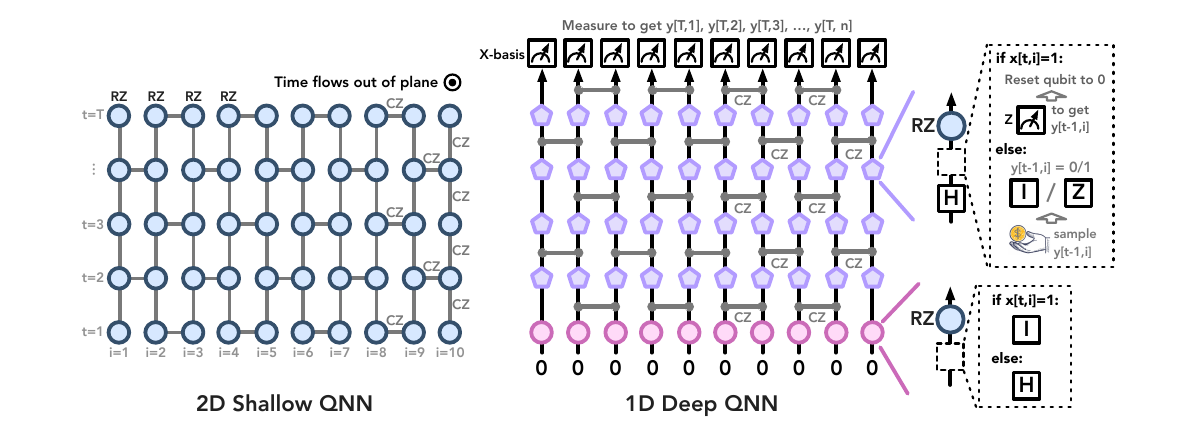
\includegraphics[width=0.79\textwidth]{assets/dqnn_idqnn_mapping.png}
  \end{center}
\end{frame}


\begin{frame}{算法一：DQNN 采样流程（深层视角）}
  设 $n=n_1m$。DQNN 只使用同一组 $m$ 个量子比特，并在 $n_1$ 个时间层上作用不同量子门。\\[0.2em]
  输入/输出采用二维索引：
  \[
    x[i_1,i_2],~y[i_1,i_2],\quad
    i_1\in\{0,\dots,n_1-1\}~(\text{时间维}),\;
    i_2\in\{1,\dots,m\}~(\text{空间维}).
  \]
  \begin{enumerate}
    \item 初始编码（$i_1=0$）：依据 $x[0,i_2]$ 对第 $i_2$ 个 qubit 编码（$0\mapsto\ket{+},\,1\mapsto\ket{0}$），得到初始乘积态 $\ket{\phi}$。
    \item 对于每个时间层，在同一组 $m$ 个 qubit 上依次施加 $R_z(\theta)$ 与层内成对 qubit 的 CZ 门，得到更新态（如 $\ket{\phi^{(1)}}$）。
    \item 对 $i_1=0,\dots,n_1-2$ 生成 $y[i_1,i_2]$ 时，分支由 $x[i_1+1,i_2]$ 决定：
    \begin{itemize}
      \item 若 $x[i_1+1,i_2]=0$：先施加 $H$，随机得到 $y[i_1,i_2]$；若结果为 1，再施加 $Z$ 校正。
      \item 若 $x[i_1+1,i_2]=1$：执行 $X$ 基测量，测量结果写入 $y[i_1,i_2]$，并将该 qubit 重置为 $\ket{0}$。
    \end{itemize}
    \item 当 $i_1=n_1-1$ 时，统一执行 $X$ 基测量，得到最后一层输出 $y[n_1-1,i_2]$。
  \end{enumerate}
\end{frame}

\begin{frame}{算法二：IDQNN（ISQNN）采样流程（浅层映射视角）}
  \begin{itemize}
    \item 使用 $n_1\times m$ 的浅层晶格结构，按 slice 组织量子比特。依据 $x[i_1,i_2]$ 对第 $(i_1,i_2)$ 个 qubit 编码（$0\mapsto\ket{+},\,1\mapsto\ket{0}$）。
    \item 每个 slice 内执行与 DQNN 对应层相同的 $R_z(\theta)$ + CZ。
    \item 相邻 slice 对应位置施加 CZ（即在 $(i_1,i_2)$ 与 $(i_1+1,i_2)$ 之间），构建跨 slice 纠缠。
    \item 逐 slice 做测量读取y并利用测量结果驱动态转移（teleportation-like update）。
    \item 对应关系：
    \[
      \text{浅层的第 }i_1\text{ 个 slice} \Longleftrightarrow
      \text{深层电路的第 }i_1\text{ 层}.
    \]
  \end{itemize}
  特点：用常深度结构实现深层随机量子电路的采样行为。
\end{frame}

\section{等价性证明}
\begin{frame}{两种电路等价性证明}
  目标是在固定输入与参数下证明：
  \[
    P_{\mathrm{IDQNN}}(y\mid x,\theta)=P_{\mathrm{DQNN}}(y\mid x,\theta).
  \]
  \vspace{0.3em}
  思路：
  \begin{itemize}
    \item 比较逐层（逐 slice）的量子态演化；
    \item 若每一步的测量分布一致，且测量后的“有效态”一致；
    \item 则最终联合输出分布 \(P(y\mid x,\theta)\) 一致。
  \end{itemize}
\end{frame}

\begin{frame}{证明}
  二维索引记号：
  \[
    x[i_1,i_2],~y[i_1,i_2],\quad
    i_1=0,\dots,n_1-1,\;\; i_2=1,\dots,m.
  \]
  \vspace{0.3em}
  记
  \[
    \ket{\psi_D^{(i_1)}}:\text{DQNN 在第 }i_1\text{ 层对应的有效态},\quad
    \ket{\psi_I^{(i_1)}}:\text{IDQNN 在第 }i_1\text{ slice 对应的有效态}.
  \]
 证明：
  \[
    \ket{\psi_D^{(i_1)}}=\ket{\psi_I^{(i_1)}}.
  \]
\end{frame}

\begin{frame}{证明结构：Base Case 与 Inductive Step}
  \textbf{Base Case（\(i_1=0\)）}
  \begin{itemize}
    \item 初始编码都由 \(x[0,i_2]\) 决定；
    \item 首层 \(R_z(\theta)\)+CZ 后，两模型有效态一致。
  \end{itemize}
  \vspace{0.2em}
  \textbf{Inductive Step（由 \(i_1\) 推到 \(i_1+1\)）}
  \begin{itemize}
    \item 假设第 \(i_1\) 步前有效态一致；
    \item 证明生成 \(y[i_1,i_2]\) 时：
    \begin{itemize}
      \item 若 \(x[i_1+1,i_2]=0\)：测量 + 前馈校正对应 teleportation 分支；
      \item 若 \(x[i_1+1,i_2]=1\)：\(X\) 基测量 + 重置对应塌缩分支；
    \end{itemize}
    \item 两分支都保持“测量分布一致 + 下一步有效态一致”。
  \end{itemize}
\end{frame}


\begin{frame}{详细展开 1：\(x[i_1+1,i_2]=0\) 分支的态演化}
  \small
  在 IDQNN 中固定第 \((i_1,i_2)\) 个 qubit。由于第 \(i_1\) 个 slice 内 CZ 门作用，它与该 slice 其余 qubit 纠缠，记
  \[
    \ket{\phi^{(i_1)}}=
    \ket{0}_{i_1,i_2}\ket{\phi_0}+\ket{1}_{i_1,i_2}\ket{\phi_1}.
  \]
  该 qubit 与 \((i_1+1,i_2)\) 位置 qubit 纠缠；当 \(x[i_1+1,i_2]=0\) 时，有
  \[
  \begin{aligned}
    \ket{\Psi}
    =&~\frac{1}{\sqrt{2}}\ket{+}_{i_1,i_2}
      \Big(\ket{+}_{i_1+1,i_2}\ket{\phi_0}
      +\ket{-}_{i_1+1,i_2}\ket{\phi_1}\Big) \\
    &+\frac{1}{\sqrt{2}}\ket{-}_{i_1,i_2}
      \Big(\ket{+}_{i_1+1,i_2}\ket{\phi_0}
      -\ket{-}_{i_1+1,i_2}\ket{\phi_1}\Big).
  \end{aligned}
  \]
  对 \((i_1,i_2)\) 做 \(X\) 测量并将结果写入 \(y[i_1,i_2]\)：
  \[
  \begin{aligned}
    y[i_1,i_2]=0 &:~ \ket{+}_{i_1+1,i_2}\ket{\phi_0}+\ket{-}_{i_1+1,i_2}\ket{\phi_1},\\
    y[i_1,i_2]=1 &:~ \ket{+}_{i_1+1,i_2}\ket{\phi_0}-\ket{-}_{i_1+1,i_2}\ket{\phi_1}.
  \end{aligned}
  \]
\end{frame}

\begin{frame}{详细展开 2：与 DQNN 的分支对齐}
  \begin{itemize}
    \item 当 \(x[i_1+1,i_2]=0\) 时,在DQNN中必须先施加门H，使状态由$\ket{0}\ket{\phi_0}+\ket{1}\ket{\phi_1}$变为$\ket{+}\ket{\phi_0}+\ket{-}\ket{\phi_1}$，与IDQNN的状态一致。
    \item 当 \(x[i_1+1,i_2]=0\) 时，若在 DQNN 中对 \(y[i_1,i_2]=1\) 的分支施加 \(Z\) 校正，则两模型后续的有效状态一致。
    \item 当 \(x[i_1+1,i_2]=1\) 时，\((i_1+1,i_2)\) 位置初始化为 \(\ket{0}\)，对应的 CZ 不改变量子态；随后对 \((i_1,i_2)\) 做 \(X\) 测量并重置，\((i_1+1,i_2)\) 的有效状态保持为 \(\ket{0}\)。
    \item 因而两种分支下，IDQNN 与 DQNN 的“测量结果分布 + 下一步有效态”均保持一致,演化轨迹保持相同。
  \end{itemize}
\end{frame}



\begin{frame}{量子优越性（对应 H.3/H.4）}
  在论文假设下（non-uniform PH 不塌缩）（没看懂）：
  \begin{itemize}
    \item 这类生成任务对量子模型是可学习且可采样的（quantumly easy）。
    \item 对经典模型则采样困难（classically hard）。
    \item 因此可支持 generative quantum advantage 。
  \end{itemize}
\end{frame}

\section{代码结果展示}

\begin{frame}{采样代码与示例}
  对应文件：
  \begin{itemize}
    \item \texttt{DQNN\_generate\_y.py}：实现 DQNN 采样流程。
    \item \texttt{IDQNN\_generate\_y.py}：实现 IDQNN 采样流程。
  \end{itemize}
  \vspace{0.3em}
   \texttt{x bitstring = "00001111000000110000" \# n=20, m=5, n1=4.}
 \begin{center}
    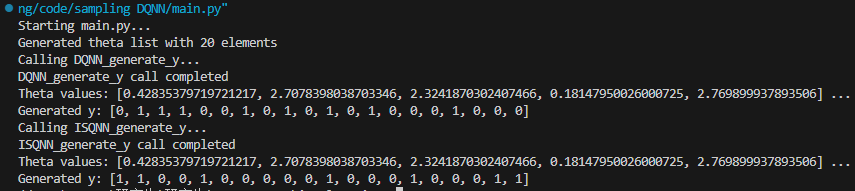
\includegraphics[width=0.92\textwidth]{assets/code_tree_screenshot.png}
  \end{center}
\end{frame}


\end{document}
